\documentclass{article}
\usepackage{graphics}
\usepackage{tikz}
\pgfrealjobname{bn2}
\begin{document}
% pdflatex --jobname=bn2-g bn2.tex
\beginpgfgraphicnamed{bn2-g}
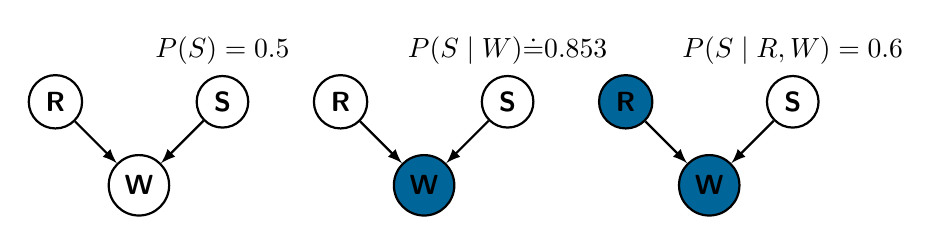
\begin{tikzpicture}[>=latex, node distance=1.5cm, every loop/.style={},
                    thick,main node/.style={circle,draw,font=\sffamily\bfseries},
                    filled/.style={circle, draw=black, fill={rgb:red,0;green,122;blue,184}}]

  \node[main node] (1) {W};
  \node[main node] (2) [above left of=1] {R};
  \node[main node] (3) [above right of=1, label=above:{$P(S) = 0.5$}] {S};
  \node[main node] (4) [right of=3] {R};
  \node[main node] (5) [filled, below right of=4] {W};
  \node[main node] (6) [above right of=5, label=above:{$P(S \mid W) \dot{=} 0.853$}] {S};
  \node[main node] (7) [filled, right of=6] {R};
  \node[main node] (8) [filled, below right of=7] {W};
  \node[main node] (9) [above right of=8, label=above:{$P(S \mid R,W) = 0.6$}] {S};

  \path[->][every node/.style={font=\sffamily\small}]
    (2) edge [left] node [left] {} (1)
    (3) edge node [left] {} (1)
    (4) edge node [] {} (5)
    (6) edge node [right] {} (5)
    (7) edge node [] {} (8)
    (9) edge node [right] {} (8);
\end{tikzpicture}
\endpgfgraphicnamed
\end{document}